\chapter{格子ボルツマン法を組み込んだ深層学習モデル\label{chap:how-to-assemble}}
この章では,提案モデルの概要とより具体的な原理について説明する.

\section{提案モデルの概要}
提案モデルの概要図を図\ref{fig:overview}に示す.この図が示すように,提案モデルはLBMをベースとしている.その並進と衝突の計算に重みを導入し,予測速度と圧力に対する実際の速度と圧力との誤差からその重みを誤差逆伝播法によって学習することで,座標に依存する流体の振る舞いを精度良くシミュレーションすることを試みる.学習の流れを詳述する.まずある時刻$t_0$の各格子点上での流体の速度,圧力から,仮想粒子の分布$f(\bm{x}, \bm{v}, t_0)$を導出する.そこから数ステップに亘り,並進と衝突の計算によって仮想粒子の分布$f'(\bm{x}, \bm{v}, t+i)$, $f(\bm{x}, \bm{v}, t+i+1) \hspace{10pt}(i=0,1,2,...)$を逐次的に得る.最終的な分布$f(\bm{x}, \bm{v}, t_1) \hspace{5pt}(t_1>t_0)$から巨視的な流体の速度と圧力を算出し,これと実際の流体の速度と圧力との誤差から,各ステップに導入した重みを誤差逆伝播法によって学習する.
\begin{figure}[htbp]
  \centering
  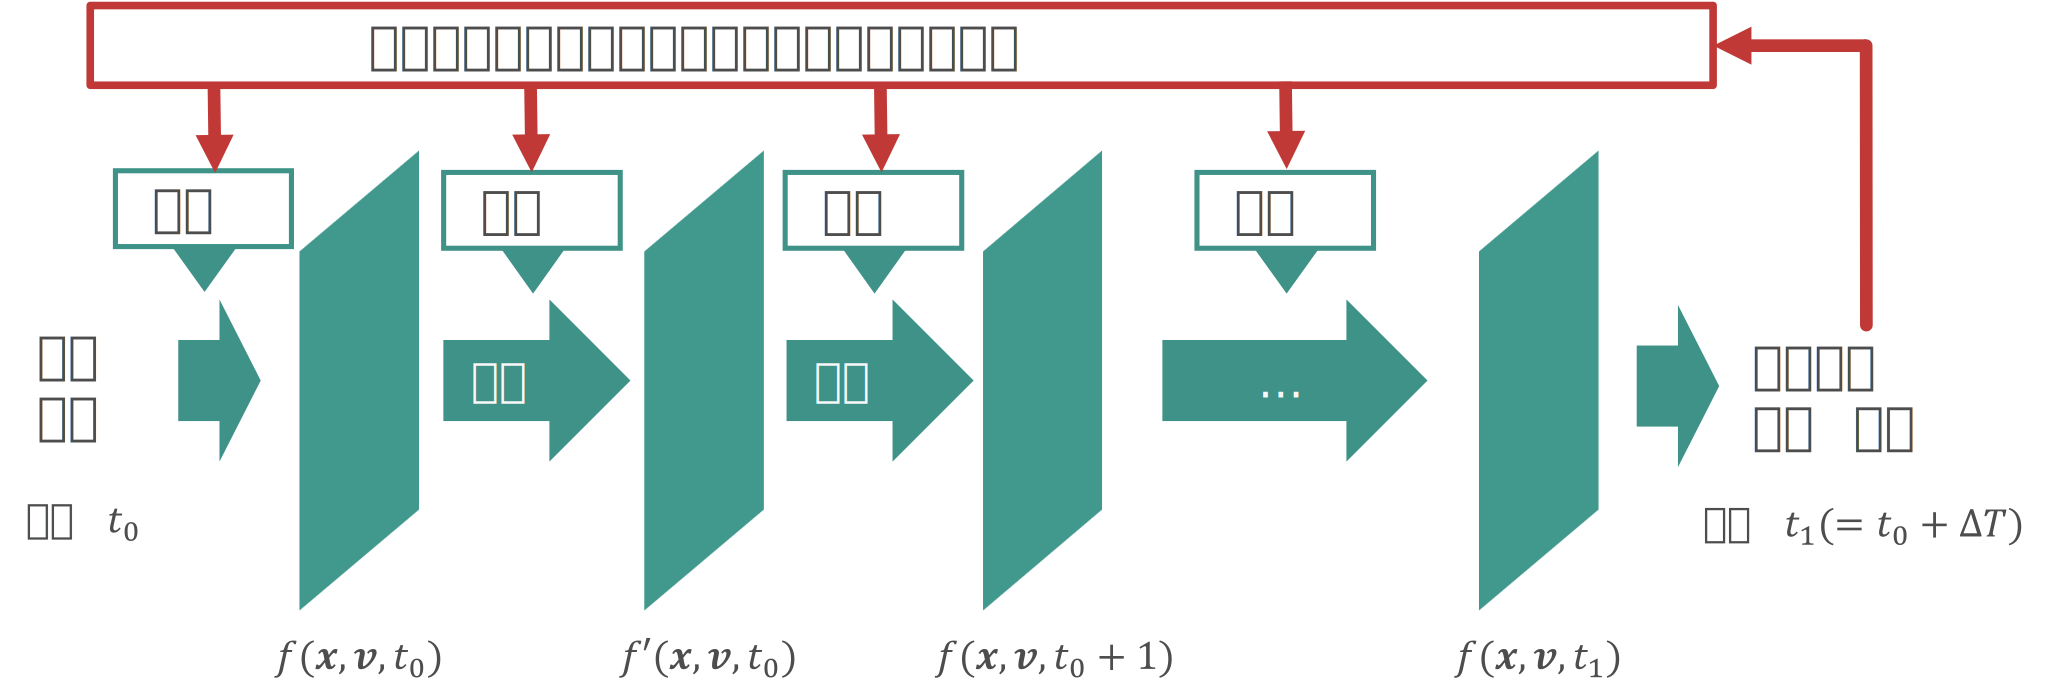
\includegraphics[width=13cm]{./how_to_assemble/figs/model_overview.svg.eps}
  \caption{提案モデルの概要図}
  \label{fig:overview}
\end{figure}

\section{提案モデルの原理}
この節では,具体的にどのようにLBMに重みを導入し学習を行うか,その原理について説明する.まずは図\ref{fig:model}(a)で表されるように,ある一時刻のデータのみが入力されたときにその3時間後の流速のみを予想する時系列性のないモデルを説明する.その後,図\ref{fig:model}(b)で表されるように3時間おきの時系列データが入力されたとき,それぞれの時刻に対して3時間後の時系列流速データを予想するモデルを説明する.

\subsection{時系列性のないモデル\label{subsection:time-series-less-model}}
LBMの並進は,仮想粒子の分布関数$f(\bm{x}, \bm{v}, t)$を用いて以下のように表された(再掲).
\begin{equation}
  f'(\bm{x}+\bm{v}, \bm{v}, t)
  = f(\bm{x}, \bm{v}, t)
  \tag{\ref{eq:principles-streaming}}
  % todo: あとで第二章の式と整合性が取れているか最終チェックする
\end{equation}

この式に重み$w'_{\rm{const}}(\bm{x}, \bm{v}, t)$, $w'_{\rm{fprev}}(\bm{x}, \bm{v}, t)$を導入する.重みを導入することで,仮想粒子の分布関数$f(\bm{x}, \bm{v}, t)$を並進させる際に,仮想粒子の流入や流出を表現することができる.重みを導入した並進の式は以下のように表される.
\begin{equation}
  f'(\bm{x}+\bm{v}, \bm{v}, t) = 
  w'_{\rm{const}}(\bm{x}, \bm{v}, t) + 
  w'_{\rm{fprev}}(\bm{x}, \bm{v}, t) f(\bm{x}, \bm{v}, t)
  \label{eq:weighted-streaming}
\end{equation}

また,衝突の式は以下のように表された(再掲).
\begin{equation}
  f(\bm{x}, \bm{v}, t+1) = 
  f'(\bm{x}, \bm{v}, t) - 
  \frac{1}{\tau} \left[ 
    f'(\bm{x}, \bm{v}, t) - f^{eq}(\bm{x}, \bm{v}, t) 
  \right]
  \tag{\ref{eq:principles-collision}}
  % todo: あとで第二章の式と整合性が取れているか最終チェックする
\end{equation}

\begin{equation}
  f^{eq}(\bm{x}, \bm{v}, t) = 
  c_i(\bm{v}) \rho'(\bm{x}, t) \left[ 
    1 
    + 3\bm{v} \cdot \bm{u}'(\bm{x}, t) 
    + \frac{9}{2}(\bm{v} \cdot \bm{u}'(\bm{x}, t))^2 
    - \frac{3}{2}\bm{u}'(\bm{x}, t)^2 
  \right]
  \tag{\ref{eq:principles-equilibrium}}
  % todo: あとで第二章の式と整合性が取れているか最終チェックする
\end{equation}

これらの式にも重み$w_{\rm{fprev}}(\bm{x}, \bm{v}, t)$, $w_{\rm{vu}}(\bm{x}, \bm{v}, t)$, $w_{\rm{vxu}}(\bm{x}, \bm{v}, t)$, $w_{\rm{vu2}}(\bm{x}, \bm{v}, t)$, $w_{\rm{u2}}(\bm{x}, \bm{v}, t)$を導入する.重みを導入した衝突の式はそれぞれ以下のように表される.
\begin{equation}
  f(\bm{x}, \bm{v}, t+1) = 
  w_{\rm{fprev}}(\bm{x}, \bm{v}, t) f'(\bm{x}, \bm{v}, t) 
  + \left(1 - w_{\rm{fprev}}(\bm{x}, \bm{v}, t)\right) f^{eq}(\bm{x}, \bm{v}, t)
  \label{eq:weighted-collision}
\end{equation}

\begin{equation}
\begin{split}
  f^{eq}(\bm{x}, \bm{v}, t) =
  &c_i(\bm{v}) \rho'(\bm{x}, t) \\
  &[ 1 + w_{\rm{vu}}(\bm{x}, \bm{v}, t)\bm{v} \cdot \bm{u}'(\bm{x}, t) \\
  &+ w_{\rm{vxu}}(\bm{x}, \bm{v}, t)\bm{v} \times \bm{u}'(\bm{x}, t) \\
  &+ w_{\rm{vu2}}(\bm{x}, \bm{v}, t)(\bm{v} \cdot \bm{u}'(\bm{x}, t))^2 \\
  &+ w_{\rm{u2}}(\bm{x}, \bm{v}, t)\bm{u}'(\bm{x}, t)^2 ]
\end{split}
  \label{eq:weighted-equilibrium}
\end{equation}

ただし,$\times$はベクトル$\bm{u} = (u_1, u_2)$, $\bm{v} = (v_1, v_2)$に対して
\begin{equation}
  \bm{u} \times \bm{v} = u_1 v_2 - u_2 v_1
  \label{eq:cross-product}
\end{equation}
と定義される演算子である.ここで,式(\ref{eq:principles-equilibrium})と比べて式(\ref{eq:weighted-equilibrium})には新たに$w_{\rm{vxu}}(\bm{x}, \bm{v}, t)\bm{v} \times \bm{u}(\bm{x}, t)$という項が導入されている.これは,座標$\bm{x}$における流体の回転を表現するためである.

次に,どのように流速と圧力のデータを入力層へと入力するか,出力層から流速と圧力のデータを取得して損失を計算するか説明する.与えられた流速と圧力のデータだけでは仮想粒子の分布状態$f(\bm{x}, \bm{v}, t)$を計算することはできないが,ここでは局所平衡分布関数に重みを導入した式(\ref{eq:weighted-equilibrium})を用いて入力層の分布状態を推定した.また,出力層では単純に仮想粒子の分布$f(\bm{x}, \bm{v}, t)$から式(\ref{todo})を用いて流速と圧力を算出した.算出した時刻$t_1$の流速$\bm{u}(\bm{x}, t_1)$と圧力$\rho(\bm{x}, t_1)$と実際の流速$\hat{\bm{u}}(\bm{x}, t_1)$と圧力$\hat{\rho}(\bm{x}, t_1)$から求められる二乗損失は,式(\ref{todo})から次のように表される.
\begin{equation}
  E = \sum_{\bm{x}} 
  \left\| \bm{u}(\bm{x}, t_1) - \hat{\bm{u}}(\bm{x}, t_1) \right\|^2 +
  \left| \rho(\bm{x}, t_1) - \hat{\rho}(\bm{x}, t_1) \right|^2
  \label{eq:error-function}
\end{equation}

以上の重みの初期値の設定として,通常のLBMと同じ係数となるように以下のように定めた.
\begin{equation}
  \left\{ \,
      \begin{aligned}
      & w'_{\rm{const}}(\bm{x}, \bm{v}, t) = 0 \\
      & w'_{\rm{fprev}}(\bm{x}, \bm{v}, t) = 1 \\
      & w_{\rm{fprev}}(\bm{x}, \bm{v}, t) = 1 - 1/\tau \\
      & w_{\rm{vu}}(\bm{x}, \bm{v}, t) = 3 \\
      & w_{\rm{vxu}}(\bm{x}, \bm{v}, t) = 0 \\
      & w_{\rm{vu2}}(\bm{x}, \bm{v}, t) = 9/2 \\
      & w_{\rm{u2}}(\bm{x}, \bm{v}, t) = -3/2
      \end{aligned}
  \right.
\end{equation}

この初期値から学習を進めることで重みを更新していく.例として,中間層の重み$w'_{\rm{fprev}}(\bm{x}, \bm{v}, t)$の更新式を示す.最も単純な勾配降下法では,式(\ref{todo}), (\ref{eq:weighted-streaming})より以下のように表される.
\begin{equation}
  w'_{\rm{fprev}}(\bm{x}, \bm{v}, t) \leftarrow
  w'_{\rm{fprev}}(\bm{x}, \bm{v}, t) 
  - \eta \delta'(\bm{x} + \bm{v}, \bm{v}, t) f(\bm{x}, \bm{v}, t)
  \label{eq:weight-fprev-update}
\end{equation}
ただし,$\delta'(\bm{x} + \bm{v}, \bm{v}, t)$は$f'(\bm{x} + \bm{v}, \bm{v}, t)$の誤差を表している(式\ref{todo}を参照).
実行する上ではpyTorchによって自動微分が行われるので,このような更新式の導出は必要ない.

注意すべき点として,式(\ref{eq:weighted-streaming})からわかるように並進をするとき最も外側の座標の仮想粒子の分布関数は算出することができない.そのため,並進をするたびに外枠一ます分の分布関数は消滅してしまうので,入力されるデータの大きさに比べて,出力されるデータの大きさは並進の回数分小さくなる(図\ref{todo}).

\subsection{時系列性のあるモデル}
実験で用いたモデルには入力データの時系列性を反映させるため,更にリカレントな重みを導入した(図\ref{todo}).まず,いくつかの記号を再定義する.時系列データの長さを$n$とする.そして無次元時刻$t_0$から$t_n$までの$\Delta t$おきの時系列データを
\begin{equation}
    \left(\hat{\bm{u}}(\bm{x}, t_0), \hat{\rho}(\bm{x}, t_0)\right),
    \left(\hat{\bm{u}}(\bm{x}, t_1), \hat{\rho}(\bm{x}, t_1)\right),
    \cdots,
    \left(\hat{\bm{u}}(\bm{x}, t_n), \hat{\rho}(\bm{x}, t_n)\right)
  \label{eq:time-series-input}
\end{equation}
ただし,
\begin{equation}
  t_i = t_0 + i \Delta t \hspace{10pt} (0 \leq i \leq n)
\end{equation}
のように表す.なお,$\hat{\bm{u}}(\bm{x}, t_i)$は実際の無次元流速,$\hat{\rho}(\bm{x}, t_i)$は実際の無次元圧力を表す($0 \leq i \leq n$).更に,時刻$t_i$のデータが入力されたときの内部における時刻$t$($t_i \leq t \leq t_{i+1}$)の衝突(並進)後の仮想粒子の分布関数とそれから式(\ref{todo})によって得られる巨視的な流速,圧力をそれぞれ
\begin{equation}
  f_i^{(\prime)}(\bm{x}, \bm{v}, t)
  \label{eq:time-series-f}
\end{equation}
\begin{equation}
  \bm{u}_i^{(\prime)}(\bm{x}, t)
  \label{eq:time-series-u}
\end{equation}
\begin{equation}
  \rho_i^{(\prime)}(\bm{x}, t)
  \label{eq:time-series-rho}
\end{equation}
と表すことにする.局所平衡分布関数$f_i^{eq}(\bm{x}, \bm{v}, t)$も同様である.
 さて,このモデルでは重みづけられた並進の式(\ref{eq:weighted-streaming})は更に重み成分$w'_{\rm{recur}}(\bm{x}, \bm{v}, t)$が加えられ次のように拡張される(ここで,各重みの変数$(\bm{x}, \bm{v}, t)$は省略してあることに注意せよ).
\begin{equation}
  f_i'(\bm{x}+\bm{v}, \bm{v}, t) =
  \begin{dcases}
    w'_{\rm{const}} + w'_{\rm{fprev}} f_i(\bm{x}, \bm{v}, t)
    & (i = 0) \\
    \begin{split}
      & w'_{\rm{recur}} f_{i-1}(\bm{x}, \bm{v}, t - \Delta t) \\
      & \qquad + (1 - w'_{\rm{recur}})
      \left(
        w'_{\rm{const}} + w'_{\rm{fprev}} f_i(\bm{x}, \bm{v}, t)
      \right)
    \end{split}
    & (0 < i \leq n-1)
  \end{dcases}
  \label{eq:weighted-streaming-time-series}
\end{equation}

続いて,重みづけられた衝突の式(\ref{eq:weighted-collision}), (\ref{eq:weighted-equilibrium})には更に重み成分$w_{\rm{recur}}(\bm{x}, \bm{v}, t)$が加えられそれぞれ次のように拡張される(こちらも各重みの変数$(\bm{x}, \bm{v}, t)$を省略した).
\begin{equation}
  f_i(\bm{x}, \bm{v}, t + 1) = \\
  \begin{dcases}
    w_{\rm{fprev}} f_i'(\bm{x}, \bm{v}, t)
    + (1 - w_{\rm{fprev}}) f_i^{eq}(\bm{x}, \bm{v}, t)
    & (i = 0) \\
    \begin{split}
      & w_{\rm{recur}} f_{i-1}(\bm{x}, \bm{v}, t - \Delta t + 1) \\
      & \hspace{5pt} + (1 - w_{\rm{recur}})
      \left(
        w_{\rm{fprev}} f_i'(\bm{x}, \bm{v}, t)
        + (1 - w_{\rm{fprev}}) f_i^{eq}(\bm{x}, \bm{v}, t)
      \right)
    \end{split}
    & (0 < i \leq n-1)
  \end{dcases}
  \label{eq:weighted-collision-time-series}
\end{equation}

\begin{equation}
\begin{split}
  f_i^{eq}(\bm{x}, \bm{v}, t) =
  &c_i(\bm{v}) \rho_i'(\bm{x}, t) \\
  &[ 1 + w_{\rm{vu}}\bm{v} \cdot \bm{u}_i'(\bm{x}, t) \\
  &+ w_{\rm{vxu}}\bm{v} \times \bm{u}_i'(\bm{x}, t) \\
  &+ w_{\rm{vu2}}(\bm{v} \cdot \bm{u}_i'(\bm{x}, t))^2 \\
  &+ w_{\rm{u2}}\bm{u}_i'(\bm{x}, t)^2 ]
\end{split}
  \label{eq:weighted-equilibrium-time-series}
\end{equation}

続いて,どのように流速と圧力の時系列データを入力層へと入力するか,出力層から流速と圧力の時系列データ
を取得し損失を計算するか説明する.図{\ref{todo}}に示すように,まず入力層に$\left(\hat{\bm{u}}(\bm{x}, t_0), \hat{\rho}(\bm{x}, t_0)\right)$.出力層では単純に仮想粒子の分布$f_i(\bm{x}, \bm{v}, t)$から式(\ref{todo})を用いて流速と圧力を算出し,実際の流速$\hat{\bm{u}}(\bm{x}, t_n)$と圧力$\hat{\rho}(\bm{x}, t_n)$から求められる二乗損失は,次のように表される.

\begin{equation}
  E = \sum_{\bm{x}} 
  \left\| \bm{u}_n(\bm{x}) - \hat{\bm{u}}(\bm{x}, t_n) \right\|^2 +
  \left| \rho_n(\bm{x}) - \hat{\rho}(\bm{x}, t_n) \right|^2
  \label{eq:error-function-time-series}
\end{equation}